%%%%%%%%%%%%%%%%%%%%%%%%%%%%%%%%%%%%%%%%%%%%%%%%%%%%%%%%%%%%%%%%%%%%%%%%
\chapter{Group-Harmonic and Group-Closeness Maximization -- Approximation and Engineering}
\label{ch:group-harm-clos-max}
% Labels: approximate, static, distance-based (closeness)
% both sequential and parallel
%%%%%%%%%%%%%%%%%%%%%%%%%%%%%%%%%%%%%%%%%%%%%%%%%%%%%%%%%%%%%%%%%%%%%%%%

\section{Introduction}
In \Cref{ch:group-closeness-local-search}, we introduced the \emph{group-closeness
maximization} problem. This problem is \np-hard and recent work focused on
heuristics~\cite{DBLP:conf/bigdataconf/AngrimanGM19,DBLP:conf/alenex/BergaminiGM18,
DBLP:conf/adc/ChenWW16}.
Heuristics, however, do not provide approximation bounds, leaving the open
question of approximability of group-closeness maximization.
The close relationship between group-closeness maximization and the metric
$k$-Median problem as well as know local search algorithms with constant-factor
approximation bounds for the latter~\cite{DBLP:journals/siamcomp/AryaGKMMP04}
motivate us to investigate whether the $k$-Median results can be transferred
not only to group-closeness maximization, but also to group-harmonic
maximization.

\paragraph{Contribution}
%
In this chapter, we illustrate how the new theoretical results presented
in~\cite{DBLP:conf/alenex/AngrimanBDGGM21} can be used to develop the first
approximation algorithms for group-harmonic and group-closeness maximization.
For group-harmonic, we implement an efficient greedy algorithm which,
as shown in~\cite{DBLP:conf/alenex/AngrimanBDGGM21}, has
approximation ratios of $\lambda(1 - 2/e)$ in directed graphs and $\lambda(1 -
1/e)/2$ in undirected graphs, where $\lambda$ is the ratio of the minimal and
the maximal edge weights.
%
Additionally, since $\gharm$ is
submodular~\cite{DBLP:conf/alenex/AngrimanBDGGM21} but not necessarily
monotone, we directly apply the local search algorithm by Lee
\etal~\cite{DBLP:journals/siamdm/LeeMNS10}, which evaluates $\Omega(n^2)$ swaps
per iteration and achieves an approximation factor of
$\frac{1 + \epsilon}{6}$.
%

Concerning group-closeness, we adapt the local search algorithm for $k$-Median
by Arya \etal~\cite{DBLP:journals/siamcomp/AryaGKMMP04} to group-closeness
maximization. The algorithm yields constant-factor approximation for undirected
graphs, whereas in directed case the approximation factor is
$\Theta(n^{-\epsilon})$, with $\epsilon < 1/2$.

In our experimental study, we show that, on small instances where an optimum can
be computed in reasonable time, the quality of both the greedy and the local
search algorithms are on average less than $0.5\%$ away from the optimum. On
larger instances, our local search algorithms yield results with superior
quality compared to existing greedy~\cite{DBLP:conf/alenex/BergaminiGM18} and
local search solutions~\cite{DBLP:conf/bigdataconf/AngrimanGM19} at the cost
of additional running time. In particular, local search is one to three orders
of magnitude slower than greedy, but this is to be expected due to a high
quality demand -- indeed, unlike the local search heuristics presented in
\Cref{ch:group-closeness-local-search}, local search approximation algorithms
often cut greedy's (empirical) gap to optimality by half or more. We thus
advocate local search approximation for scenarios where solution quality is of
highest concern.
%The algorithm starts from an initial group $S$, and exchanges vertices from $S$ and
%$V \setminus S$. An exchange is done only if $cost(S') \le (1 - \epsilon / Q)
%\cdot cost(S)$, where $S'$ is the group after the exchange, $Q$ is the number
%of neighboring solutions -- \ie how many different $S'$ are one exchange away
%from $S$, and $\epsilon > 0$.


\bibnotes{The contributions
presented in this chapter were published in the
Proceedings of the \alenex{Twenty-Third}{2021}.
My contributions involve the engineering improvements
(\Cref{sec:gh-gc:algo-eng}), the implementation of all presented algorithms, and
carrying out the experiments.
The rest is joint work with Ruben Becker, Gianlorenzo D'Angelo, Hugo Gilbert,
Alexander van der Grinten, and Henning Meyerhenke.
Proofs to which I did not contribute are omitted and can be
found in the original paper~\cite{DBLP:conf/alenex/AngrimanBDGGM21}.}

\section{Preliminaries}
%
Recall from \Cref{sec:group-centrality-measures} the definitions of group-harmonic
and group-closeness centrality of a group $S \subset V$, namely:
$\gclos(S) := \frac{n}{\sum_{u \in V \setminus S}d(S, u)}$ and
$\gharm(S) := \sum_{u \in V \setminus S}\frac{1}{d(S, u)}$, where
$\frac{1}{d(S, u)} = 0$ if there is no
path from $S$ to $u$.

\paragraph{Problems Addressed}
%
In this chapter, we address the problems of finding groups with size $1 \le k < n$
that maximize group-harmonic and group-closeness, more formally:

\begin{minipage}[t]{.45\textwidth}
\begin{cproblem}{Group-Harmonic Maximization}
\begin{tabular}{ll}
\textbf{Input:} & Graph $G = (V, E, w)$,\\
                & integer $1 \le k < n$.\\
\textbf{Find:} & Set $S^\star \subset V$ with $|S| = k$ s.t.\\
               & $\gharm(S^\star)$ is maximum.
\end{tabular}
\end{cproblem}
\end{minipage}\hfill
\begin{minipage}[t]{.45\textwidth}
\begin{cproblem}{Group-Closeness Maximization}
\begin{tabular}{ll}
\textbf{Input:} & Graph $G = (V, E, w)$,\\
                & integer $1 \le k < n$.\\
\textbf{Find:} & Set $S^\star \subset V$ with $|S| = k$ s.t.\\
               & $\gclos(S^\star)$ is maximum.
\end{tabular}
\end{cproblem}
\end{minipage}\vspace{\baselineskip}

While group-closeness maximization has already been studied in other
works~\cite{DBLP:conf/alenex/BergaminiGM18,DBLP:conf/bigdataconf/AngrimanGM19,DBLP:conf/adc/ChenWW16},
to the best of our knowledge, we are the first to study the group-harmonic
maximization problem.

In both problems we study, we are given a (possibly directed) weighted
graph $G = (V, E, w)$ with weight function $w : E \to \natn_{> 0}$. For
group-closeness maximization, we assume that $G$ is (strongly) connected,
whereas for group-harmonic we only assume that there are no isolated vertices.
Further, we denote by
$\wmin := \min_{e \in E} w(e)$ and $\wmax := \max_{e \in E} w(e)$ the lowest
and the highest edge weights, respectively, and by $\lambda :=
\frac{\wmin}{\wmax}$ the ratio of the smallest and the
largest edge weights.


\section{Group-Harmonic Maximization}
\subsection{Mathematical Properties}
\label{sec:gh-gc-gh-math-prop}

First of all we consider the mathematical properties of $\gharm$.
We observe that the function is submodular but not monotone.

\begin{lemma}
The function $\gharm : 2^V \to \ratn_{\ge 0}$ is
submodular~\cite[Lemma 3.1]{DBLP:conf/alenex/AngrimanBDGGM21}.
\end{lemma}

The non-monotonicity of $\gharm$ can be shown with a counterexample:
consider an undirected graph with $V = \set{u, v}$ and $E = \set{\set{u, v}}$;
we have that $\gharm(\set{u}) = 1$, while $\gharm(\set{u, v}) = 0$.

\subsection{Approximation Algorithms}
%
\begin{algorithm}[tb]
\caption{Greedy algorithm for maximizing a monotone submodular set function $f$
under a cardinality constraint $|S| = k$.}
\label{algo:gh-greedy}
\begin{algorithmic}[1]
\State$S \gets \emptyset$
\While{$|S| < k$}
\State$u \gets \argmax_{v \in V \setminus S}\set{f(S \cup \set{v}) - f(S)}$
\State$S \gets S\cup\set{v}$
\EndWhile
\State\Return$S$
\end{algorithmic}
\end{algorithm}



As $\gharm$ is submodular, we can directly apply the algorithm by Lee
\etal~\cite{DBLP:journals/siamdm/LeeMNS10} and obtain a
$(\frac{1 + \epsilon}{6})$-approximation -- the exact cardinality
constraint corresponds to the case of a single matroid base constraint,
where the matroid is the uniform one.
This algorithm was notably improved by
Vondr\'ak~\cite{DBLP:conf/focs/Vondrak09}, who
designed a randomized local search method with an approximation factor
of $\frac{1}{4} - o(1)$.
Another candidate approximation algorithm for group-harmonic maximization
is the greedy algorithm (see \Cref{algo:gh-greedy}). It provides an
approximation factor of $1 - \frac{1}{e}$ for maximizing a monotone and
submodular set function under a cardinality constraint $|S| = k$.
However, as observed in \Cref{sec:gh-gc-gh-math-prop}, $\gharm$ is not
monotone and we cannot use this result directly.
\Cref{algo:gh-greedy} still guarantees approximation bounds nonetheless, they
are summarized in the following Theorem.

\begin{theorem}[\cite{DBLP:conf/alenex/AngrimanBDGGM21}]
    \Cref{algo:gh-greedy} guarantees the following approximation factor for the
    group-harmonic maximization problem, where $\lambda := \frac{\wmin}{\wmax}$
    is the ratio of the minimum and the maximum edge weights:
    \begin{itemize}
        \item$\lambda\roundb{1 - \frac 2e} > 0.264\lambda$ in the directed case;
        \item$\frac \lambda2\roundb{1 - \frac 1e} > 0.316\lambda$ in the undirected case.
    \end{itemize}
\end{theorem}

While these approximation factors may be worse than the ones provided by
Lee \etal~\cite{DBLP:journals/siamdm/LeeMNS10} and
Vondr\'ak~\cite{DBLP:conf/focs/Vondrak09}, they offer better guarantees
for the group-harmonic maximization problem in unweighted graphs.

\begin{lemma}[\cite{DBLP:conf/alenex/AngrimanBDGGM21}]
If $G$ is unweighted, then the set returned by \Cref{algo:gh-greedy}
provides a $\frac 12\roundb{1 - \frac 1e}$-approximation.
\end{lemma}

\subsection{Engineering Improvements}
\label{sec:gh-gc:algo-eng}
%
In the following, we illustrate engineering techniques to accelerate the greedy
and the local search algorithms for group-harmonic maximization.

\paragraph{Greedy Algorithm}
%
\begin{algorithm}[tb]
\footnotesize
\caption{\footnotesize Greedy algorithm for group-harmonic maximization.}
\label{algo:gh-greedy-eng}
\begin{algorithmic}[1]
\State$top_h \gets \texttt{topHarmonicCloseness}()$~\cite{DBLP:conf/alenex/BiseniusBAM18}
\label{line:gh-greedy-eng:toph}
\State$S \gets \set{top_h}$
\While{$|S| < k$}
\State$PQ \gets$ max-priority queue with key $\gharmupp(S, u)$ and value $u$
\label{line:gh-greedy-eng:lg-1}
\For{\textbf{each} $u \in V \setminus S$}
\State$PQ.\texttt{push}(u)$
\EndFor
\State$x \gets \nil$\Comment{Vertex with highest marginal gain computed so far}
\State$\gharm(S\cup\set{x}) \gets -\infty$\smallskip

\Repeat\Comment{This loop is done in parallel}
\State$u \gets PQ.\texttt{extractMax}()$
\If{$\gharmupp(S, u) \le \gharm(S \cup \set{x})$}
\State\textbf{break}\Comment{$x$ has the highest marginal gain}
\EndIf
\State$\left<\isexact, \gharm(S \cup \set{u})\right> \gets$
pruned SSSP$(u, \gharm(S \cup\set{x}))$
\label{line:gh-greedy-eng:pruned-sssp}
\If{\isexact \textbf{and} $\gharm(S\cup\set{u}) > \gharm(S \cup \set{x})$}
\State$x \gets u$
\EndIf
\Until{$PQ$ is empty}
\State$S \gets S \cup \set{x}$
\label{line:gh-greedy-eng:lg-2}
\EndWhile
\State\Return$S$
\end{algorithmic}
\end{algorithm}


The pseudocode of our greedy algorithm is given by \Cref{algo:gh-greedy-eng}.
The first vertex to be added to the group is the vertex with highest
harmonic centrality (\Cref{line:gh-greedy-eng:toph}); this vertex can be
found by a ranking algorithm such as the one from Bisenius
\etal~\cite{DBLP:conf/alenex/BiseniusBAM18}. Afterwards, the algorithm
iteratively adds to the group the vertex $u$ with highest marginal gain
$\gharm(S \cup \set{u}) - \gharm(S)$.

Since $\gharm$ is submodular, we can evaluate marginal gains lazily,
\ie the marginal gain from previous iterations $\gharmupp(S, u)$ serves
as an upper bound of the marginal gain $\gharm(S \cup \set{u}) - \gharm(S)$
in the current iteration. Since $\gharmupp(S, u) \ge \gharm(S\cup\set{u})$
holds after $S$ is initialized with the vertex with highest harmonic
centrality, we initialize $\gharmupp(S, u)$ to $\harmupp(u)$ for each
$u \in V \setminus S$, that is the upper bound on $\harm(u)$ computed
by the Bisenius \etal algorithm~\cite{DBLP:conf/alenex/BiseniusBAM18}.
To determine the vertex with highest marginal gain, we use the well-known
lazy strategy~\cite{minoux1978accelerated}: we evaluate the marginal
gain of the vertex with highest upper bound -- and adjust the upper bound
to the true marginal gain -- until we know the true marginal gain of the
top vertex \wrt the upper bound
(\Crefrange{line:gh-greedy-eng:lg-1}{line:gh-greedy-eng:lg-2}
of \Cref{algo:gh-greedy-eng}, by using a priority queue).

To evaluate the marginal gain of a vertex $u$, we run a pruned
SSSP from $u$ (\Cref{line:gh-greedy-eng:pruned-sssp}) that only
visits vertices $v$ such that $d(u, v) < d(S, v)$ and updates
$\gharmupp(S, u)$ after every vertex at distance $i$ from $u$
has been explored. The traversal is interrupted if
$\gharmupp(S, u) \le \gharm(S \cup \set{x})$, where $x$ is the
vertex with highest marginal gain computed so far; otherwise, the
SSSP visits all the vertices that are closer to $u$ than to $S$ and
returns the exact value of $\gharm(S \cup \set{u})$.
As for group-closeness, $\gharmupp$ is defined differently for
weighted than for unweighted graphs.

\paragraph{Pruning -- Unweighted Graphs}
%
In unweighted graphs, we exploit additional bounds to interrupt the
SSSP earlier. Let us assume that the pruned SSSP -- \ie a BFS --
has explored all vertices up to distance $i$. We denote be
$\PhiSu^{\le i}$ the set of vertices $v$ such that $d(u, v) \le i$
and $d(u, v) < d(S, v)$, with $\PhiSu^i$ the set of vertices $v$
such that $d(u, v) = i$ and $d(u, v) < d(S, v)$ and with $n_{S, u}^i$ its
cardinality. An additional upper bound on the marginal gain of $u$ is:
%
\begin{equation}
\label{eq:gh-gc-nbound}
\sum_{v \in \PhiSu^{\le i}\setminus \set{u}}
\roundb{\frac{1}{d(u, v)} - \frac{1}{d(S, v)}} +
\frac{\tilde{n}_{S, u}^{i + 1}}{i + 1} + \frac{r(u) - |\PhiSu^{\le i}| - \tilde{n}_{S, u}^{i + 1}}{i + 2} -
\frac{1}{d(S, u)}.
\end{equation}

The first summand is the contribution to the marginal gain due to the explored
vertices up to distance $i$. In the second summand, we assume that
$\tilde{n}_{S, u}^{i + 1} \ge n_{S, u}^{i + 1}$ vertices are at distance exactly
$i + 1$ from $u$, where $\tilde{n}_{S, u}^{i + 1}$ is defined as
$\sum_{x \in \PhiSu^i}\degout(x)$ for directed graphs and
$\sum_{x \in \PhiSu^i}(\deg(x) - 1)$ for undirected graphs.\footnote{As done
with upper bound for \nbcut in \Cref{eq:nbcut-bound}, a tighter numerator of
the second summand of \Cref{eq:gh-gc-nbound} is $\min(n - n_{S, u}^i,
\tilde{n}_{S, u}^{i + 1})$. However, to simplify our notation, we keep writing
$\tilde{n}_{S, u}^{i + 1}$ in the text,
but implement the better bound in practice.}
In the third summand we assume that all the remaining vertices reachable from $u$
are at distance $i + 2$ from $u$ -- recall that $r(u)$ is the number of vertices
reachable from $u$.\footnote{Because in directed graphs it is too expensive to compute
$r(u)$ for each vertex, we use an upper bound as described
in~\cite{DBLP:journals/tkdd/BergaminiBCMM19}.} Finally, we subtract the contribution
of $u$ to the centrality of $S$.

As a further optimization for unweighted and undirected graphs, for every vertex
$u \in V \setminus S$ we subtract from $r(u)$ all the vertices in $u$'s connected
component that are at distance $1$ from $S$.
In this way, we avoid to count them in the third summand of \Cref{eq:gh-gc-nbound}.


\paragraph{Pruning -- Weighted Graphs}
%
In weighted graphs, the SSSP is a pruned version of the Dijkstra algorithm. Let
$i$ be the distance from $u$ to the last explored vertex. Upon completion of
Dijkstra's relaxation step, $\gharmupp(S, u)$ is updated as follows:
%
\begin{equation}
\label{eq:gh-gc-gharmupp-update}
\gharmupp(S, u) =
\sum_{v\in \PhiSu^{\le i} \setminus \set{u}}\roundb{\frac{1}{d(u, v)} - \frac{1}{d(S, v)}} +
\frac{r(u) - |\PhiSu^{\le i}|}{i} - \frac{1}{d(S, u)},
\end{equation}
%
\ie we count the contribution to $\gharmupp(S, u)$ of (i) the vertices visited
by the SSSP and of (ii) the unexplored vertices assuming that they are all at
distance $i$ from $u$.

\paragraph{Local Search}
%
The local search algorithm by Lee \etal~\cite{DBLP:journals/siamdm/LeeMNS10}
needs to evaluate $\Omega(n^2)$ swaps per iteration. This is already quite expensive,
so it is desirable to perform only few iterations. To this end, we initialize the local
search with a greedy solution -- this does not affect its approximation guarantee but
accelerates the algorithm considerably in practice.

Although we cannot use lazy evaluation for local search -- we need to consider swaps,
not vertex additions -- we can still make use of the bound from \Cref{eq:gh-gc-nbound}
while evaluating a swap.

\paragraph{Parallelism}
%
Both greedy and local search typically need to evaluate either the
marginal gains or the objective function for several vertices before performing
a single addition (or swap). Since these evaluations are independent \change{of} each
other, it is desirable to utilize parallelism. We parallelize multiple evaluations
of the objective function in a straightforward way: Each thread evaluates the marginal
gain for one candidate vertex; this incurs of $\Oh(n)$ additional memory per thread
as it needs to store the state of a single SSSP.


\section{Group-Closeness Maximization}
\subsection{Preliminary Discussion}
\label{sec:group-harm-clos-max:gc-prel-disc}
%
Different variants of the group-closeness maximization problem occur depending
on whether the graph at hand is undirected or directed.
From an approximation algorithm's perspective, it is tempting to observe that
the group-farness $\gfarn$ is a supermodular set function and conclude that
$\gclos$ is submodular. In the literature, this argument was used in the paper
by Chen \etal~\cite{DBLP:conf/adc/ChenWW16}. Unfortunately, this approach is
flawed because the reciprocal of a supermodular set function is not necessarily
submodular and the approximation question remains unanswered. Indeed, as shown
in \Cref{lemma:prelim:gclos-not-submod}, $\gclos$ is not submodular.

A similar, yet not flawed, strategy was taken by Li
\etal~\cite{DBLP:conf/www/0002PSYZ19}. In they work they deal with the
current-flow closeness centrality -- also known as electrical closeness, see
\Cref{sec:centrality-measures} -- and they measure the approximation factor
of their algorithms in a different way, allowing them to obtain
constant-factor approximation results.
As argued in Ref.~\cite[Appendix C]{DBLP:conf/alenex/AngrimanBDGGM21}, an
analogous approach can be applied in our setting, yielding constant-factor
approximation algorithms for group-closeness maximization in their sense
(see \Cref{apx:gh-gc:li-etal-apx} for further details).
We remark, however, that the notion of approximation used by Li \etal is a
fundamentally different notion of approximation.

\subsection{Approximation Algorithms}
%
We start by introducing the metric $k$-Median problem and how we adapt it to our setting.

\begin{cproblem}{Metric $k$-Median}
\begin{tabular}{ll}
\textbf{Input:} & Set of clients $C$, set of facilities $F$, cost function $c : C \times F \to \real_{\ge 0}$
satisfying\\
                & triangle inequality, integer $k$.\\
\textbf{Find:} & Set $S \subseteq F$ with $|S| \le k$ s.t. $c(S) := \sum_{i \in C}\min_{j\in S}c(i, j)$
is minimum.
\end{tabular}
\end{cproblem}

Arya \etal~\cite{DBLP:journals/siamcomp/AryaGKMMP04} show that the local search algorithm
that performs $p$ swaps at each step leads to a solution with approximation ratio
at most $3 + 2/p$ for Metric $k$-Median.

The \emph{group-farness minimization} problem can be seen as a special case of the metric
$k$-Median problem where $C$ and $F$ are both taken to be the vertex set $V$ and
the cost function being obtained using the shortest-path distances. Since $\gfarn$
is monotone, the result of Arya \etal carries over to the undirected group-farness
minimization problem with exact cardinality constraint, yielding an approximation factor
of $\frac{p}{3p + 2}$ for group-closeness maximization.

\subsection{Engineering Improvements}
%

Since the greedy algorithm for group-closeness has already been studied
before~\cite{DBLP:conf/alenex/BergaminiGM18}, in the following, we discuss
local search and engineering improvements.

\paragraph{Local Search}
%
We consider the local search algorithm that, at each iteration, evaluates all
possible pairs of swaps. For the $k$-Median case, Arya
\etal~\cite{DBLP:journals/siamcomp/AryaGKMMP04} minimize the cost function of an
initial solution $S$. A swap is done only if $c(S') \le (1 - \epsilon/Q)\cdot c(S)$,
where $S'$ is the solution after the swap, $Q$ is the number of neighboring solutions
-- \ie how many different $S'$ are one swap away from $S$ -- and $\epsilon > 0$.
For group-closeness, the cost function is represented by $\gfarn$ -- minimum farness
is maximum closeness -- and $Q$ is $k(n - k)$, \ie the number of possible
swaps. The algorithm has an approximation ratio of 5.

Like in the group-harmonic case, the local search algorithm is much faster in practice
if we start from a good initial solution. To this end, we use the \growshrink
algorithm described in \Cref{sec:lsh-gc-grow-shrink} which, despite being heuristic,
in real-world graphs it quickly finds high-quality solutions. The lack of approximation
ratio in \growshrink is not an issue in our case, the approximation guarantee of our
local search does not depend on the initial solution.

\begin{algorithm}[t]
\footnotesize
\setstretch{1}
\caption{\footnotesize Overview of the single-swap algorithm for group-closeness maximization.}
\label{algo:gc-ls-apx}
\begin{algorithmic}[1]
\State$S \gets \growshrink(G, k)$
\State$\gfarn(S) \gets$ SSSP$(S)$
\Repeat
\State$PQ_u \gets$ min-priority queue with key $(\gfarn(S \setminus \set{u}) - \gfarn(S)$
and value $u$\label{line:gc-ls-apx:pqu1}
\For{\textbf{each} $x \in S$}
\State$PQ_u.\texttt{push}(x)$
\EndFor\label{line:gc-ls-apx:pqu2}
\State$\didswap \gets \false$
\Repeat
\State$u \gets PQ_u.\texttt{extractMin}()$
\TopComment{Compute the exact farness increase}
\State$\gfarn^+(u) \gets \gfarn(S \setminus \set{u}) - \gfarn(S)$\label{line:gc-ls-apx:gfarnplus}
\State compute $\gfarnapx((S \cup \set{v}) \setminus \set{u})$ for all $v \in V \setminus S$
\State$PQ_v \gets$ max-priority queue with key $\gfarnapx((S \cup \set{v}) \setminus \set{u})$
and value $v$\label{line:gc-ls-apx:pqv1}
\For{\textbf{each} $x \in V \setminus S$}
\State$PQ_v.\texttt{push}(x)$
\EndFor\label{line:gc-ls-apx:pqv2}
\Repeat
\State$v \gets PQ_v.\texttt{extractMax}()$
\TopComment{Compute the exact farness decrease}
\State$\gfarn((S \cup \set{v}) \setminus \set{u}) \gets$ pruned SSSP from $v$
\If{$\gfarn((S \cup \set{v}) \setminus \set{u}) \le \roundb{1 - \frac{\epsilon}{k (n - k)}}\gfarn(S)$}
\State$S \gets (S \cup \set{v}) \setminus \set{u}$
\State$\gfarn(S) \gets$ SSSP$(S)$
\State$\didswap \gets \true$
\State\textbf{break}
\EndIf
\Until{$PQ_v$ is empty}
\If{\didswap}
\State\textbf{break}
\EndIf
\Until{$PQ_u$ is empty}
\Until{not \didswap}
\State\Return$S$
\end{algorithmic}
\end{algorithm}


\paragraph{Prioritizing Swaps}
%
The actual number of swaps that need to be evaluated before a local optimum is
reached is heavily affected by the sequence of swaps that are done.
\Cref{algo:gc-ls-apx} summarizes how we prioritize the swaps. Similarly to
\growshrink, we prioritize swaps depending on their estimated impact on
$\gfarn(S)$. First, we sort in ascending order the vertices in $S$ by
the increase in $\gfarn$ due to their removal from $S$, \ie
$\gfarn(S\setminus \set{u}) - \gfarn(S)$ for all $u \in S$
(\Crefrange{line:gc-ls-apx:pqu1}{line:gc-ls-apx:pqu2} of the pseudocode).
Afterwards, in \Crefrange{line:gc-ls-apx:pqv1}{line:gc-ls-apx:pqv2}, we
sort in descending order all the vertices $v \in V \setminus S$ by
$\gfarnapx((S \cup \set{v}) \setminus \set{u})$, which is an estimate of the
decrease in farness, \ie $\gfarn((S \cup \set{v}) \setminus \set{u}) -
\gfarn(S)$.
We use the same estimate based on the size of the shortest path DAGs as described
in \Cref{ch:group-closeness-local-search}.

As a further optimization, we exclude swaps with vertices in $V \setminus S$ with
degree 1 because, in (strongly) connected graphs, they cannot result in a decrease
in $\gfarn$.

\paragraph{Additional Pruning}
%
Recall from \Cref{sec:lsh-gc-grow-shrink} that the \growshrink algorithm performs
a pruned SSSP to evaluate whether a swap is advantageous. We modify the algorithm
to incorporate additional pruning conditions that interrupt the SSSP when a swap
is not good enough to be considered in the local search -- in contrast, \growshrink
performs any swap that improves the objective function, regardless of the difference
in score. Specifically, we maintain a lower bound
$\gfarnupp(S, u, v) \le \gfarn((S \cup \set{v}) \setminus \set{u})$ so that we can
interrupt the pruned SSSP as soon as
$\gfarnupp(S, u, v) > \roundb{1 - \frac{\epsilon}{k (n - k)}}\gfarn(S)$.

$\gfarnupp(S, u, v)$ is computed in two steps: we first compute
$\gfarn^+(S, u) := \gfarn(S \setminus \set{u}) - \gfarn(S)$ exactly (\Cref{line:gc-ls-apx:gfarnplus}
in \Cref{algo:gc-ls-apx}) that is, the increase in farness of $S$ due to the
removal of $u$. Then, during every pruned SSSP from $v$, we keep updating an upper bound
of the decrease in farness of $S \setminus \set{v}$ due to the addition of $v$:
$\gfarnupp^-(S, v) := \gfarn(S \setminus \set{u}) - \gfarnupp(S, u, v)$.
Then, $\gfarnupp(S, u, v)$ is computed as $\gfarn(S) + \gfarn^+(S, u) - \gfarnupp^-(S, v)$.

To compute $\gfarn^+(S, u)$ exactly we maintain the following information
for each vertex $x \in V \setminus S$: the distance $d(S, x)$,
a representative vertex $r_x \in S$ such that $d(r_x, x) = d(S, x)$,
and the distance $d'(S, x) = d(S \setminus \set{r_x}, x)$. In this way,
$\gfarn^+(S, u)$ can be computed in $\Oh(n)$ time as done by the original
\growshrink algorithm:
%
\[
\gfarn^+(S, u) = \sum_{x \in \set{V \setminus S : d(S, x) = d(u, x)}}d(S, x) - d(S', x).
\]

$\gfarnupp^-(S, v)$ is computed differently in unweighted and weighted graphs.
In unweighted graphs, the pruned SSSP is a BFS, and we define bounds inspired by
the ones used for top-$k$ closeness centrality in Ref.~\cite{DBLP:journals/tkdd/BergaminiBCMM19}:
For every distance $1 \le i \le \diam(G)$ we maintain $N_{\ge i}(S)$, \ie the set
of vertices at distance $\ge i$ from $S$, and $\PhiSv^{\le i}$, \ie the set of vertices
$x$ such that $d(v, x) \le i$ and $d(v, x) < d(S, x)$.
%
Once every vertex in $\PhiSv^{\le i}$ has been visited by the pruned BFS, we know
that at most $\tilde{n}_{i + 1}(v) := \min\roundb{|N_{\ge i + 2}(S)|,
\sum_{x\in \PhiSv^i}\degout(x)}$ vertices can be at distance $i + 1$ from $v$,
while the remaining unexplored vertices will
be at least at distance $i + 2$ -- in undirected graphs,
$\tilde{n}_{i + 1}(v) := \min\roundb{|N_{\ge i + 2}(S)|, \sum_{x \in \PhiSv^i}(\deg(x) - 1)}$.
This, we update $\gfarnupp^-(S,  v)$ as follows:

\begin{align*}
\gfarnupp^-(S, v) =& \sum_{x \in \PhiSv^{\le i}}\roundb{d(S, x) - d(v, x)}\ +\\
                &\sum_{x \in \Lambda}(d(S, x) - i - 1) +
\sum_{x \in N_{i \ge 3}(S)\setminus\Lambda}\roundb{d(S, x) - i - 2}.
\end{align*}

The first summand represents the decrease in farness due to the vertices that have already
been visited by the BFS. In the second summand, $\Lambda \subseteq N_{\ge i + 2}(S)$ contains
the $\tilde{n}_{i + 1}(v)$ vertices closest to $S$, and we assume that they are at distance
$i + 1$ from $v$.\footnote{This assumption is done in order to consider
the \enquote{worst-case scenario} (in terms of decrease in farness) where
the vertices ad distance $i + 1$ from $v$ are also the closest ones to $S$.}
Finally, in the third summand we assume that all the remaining unvisited vertices are
at distance $\ge i + 3$ from $S$ and not counted in $\Lambda$ can be reachable from $v$
in $i + 2$ hops. From the third summand we exclude vertices at distance $i + 2$
from $S$ because, under our assumption, their distance from $S$ would remain
unchanged.
At the cost of additional $\Oh(\diam(G))$ space, $\gfarnupp^-(S, v)$ can be computed
in $\Oh(\diam(G))$ time.

For weighted graphs, we update $\gfarnupp^-(S, v)$ by adapting our strategy from \gharm
to \gfarn (see \Cref{eq:gh-gc-gharmupp-update}).

\paragraph{Parallelism}
%
We employ the same parallelization technique as for group-harmonic maximization. The
fact that in the greedy and local search algorithms evaluations of the objective function
can be parallelized can be seen as an advantage over the \growshrink algorithm which, in turn,
is inherently sequential.

\section{Experiments}
%
We conduct experiments to evaluate our algorithms in terms of solution quality and running time.
For group-harmonic, we first evaluate the quality of our greedy algorithm (\greedyh),
our local search algorithm that starts from a greedy solution (\greedylsh), and the best
over 100 sets selected uniformly at random (\bestrandomh) against the optimal
solution on small-sized networks. Then, we measure the quality and the running time
performance of \greedyh and \greedylsh and we use \bestrandomh as baseline.

Regarding group-closeness, we compare our local search algorithm against the
greedy algorithm by Bergamini \etal~\cite{DBLP:conf/alenex/BergaminiGM18}, the
\growshrink algorithm (see \Cref{ch:group-closeness-local-search}),\footnote{We
use the extended variant of \growshrink with $p = \numprint{0.75}$. As
discussed in \Cref{sec:lsh-gc-exp-extended-gs},
it achieves a reasonable time-quality trade-off.} and the best of 100 randomly
chosen sets. Hereafter, these algorithms are referred to as \greedyc, \gs, and
\bestrandomc, respectively.
%
Our local search algorithm for group-closeness uses either \greedyc or \gs
to initialize the initial solution: in the former case we label it as
\greedylsc, and \gslsc in the latter.

\subsection{Settings}
%
We implement all algorithms in C++ using the NetworKit~\cite{DBLP:journals/netsci/StaudtSM16}
graph APIs and we use SCIP~\cite{gamrath2020scip} to solve ILP instances.
All experiments are conducted on a Linux machine with an \CPU and \RAM,
and managed by the SimexPal~\cite{DBLP:journals/algorithms/AngrimanGLMNPT19}
software for reproducibility. We aggregate approximation ratios and speedups
using the geometric mean. All experiments have a timeout of one hour.

\subsection{Instances Statistics}
%
\paragraph{Datasets}
Experiments are executed on real-world complex and high-diameter networks
reported in
\Crefrange{tab:gh-gc-apx:small-inst-gh}{tab:gh-gc-apx:large-inst-gc},
\Cref{sec:gh-gc:inst-stats}. In the \enquote{Type} columns, the first letter
indicates whether the network is
undirected (\texttt{U}) or directed (\texttt{D}), while the second letter
whether the network is unweighted (\texttt{U}) or weighted (\texttt{W}).

Instances have been downloaded from the public repositories
KONECT~\cite{kunegis2013konect}, OpenStreetMap~\cite{OpenStreetMap} (from
which we build the car routing graph using
RoutingKit~\cite{DBLP:journals/jea/DibbeltSW16}) and from the 9th DIMACS
Implementation Challenge~\cite{demetrescu2009shortest}. Small instances used
for the experiments with the ILP solver are reported in
\Cref{tab:gh-gc-apx:small-inst-gh,tab:gh-gc-apx:small-inst-gc}, while the rest
of the experiments are conducted on the instances in
\Cref{tab:gh-gc-apx:large-inst-gh,tab:gh-gc-apx:large-inst-gc}.

Because algorithms for group-closeness maximization only handle (strongly)
connected graphs, we run them on the (strongly) connected components of the
instances of our datasets. For high-diameter networks, we test mainly road
networks because they are the most common type of networks in the
aforementioned repositories. We are confident, however, that our local search
algorithms are capable of handling other types of high-diameter networks
as well without significant difference in performance.
Because public repositories do not provide a reasonable amount of
\emph{weighted} complex networks, we omit these networks from our experiments.

\subsection{Group-Harmonic Maximization}
\label{sec:gh-gc:exp-gh-max}
\paragraph{Comparison to Exact ILP Solutions}
%
\begin{figure}[tb]
\begin{subfigure}[t]{\textwidth}
\centering

\includegraphics{./sources/plots/gh-gc-apx/legend-exact-harmonic.pdf}
\end{subfigure}\medskip

\begin{subfigure}[t]{.5\textwidth}
\centering
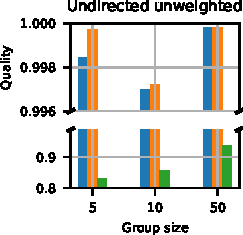
\includegraphics[width=.49\textwidth]{./sources/plots/gh-gc-apx/quality-ilp-harmonic-small-diameter-undirected-unweighted.pdf}
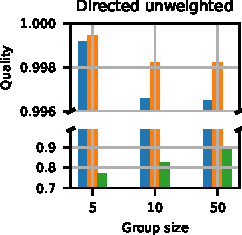
\includegraphics[width=.49\textwidth]{./sources/plots/gh-gc-apx/quality-ilp-harmonic-small-diameter-directed-unweighted.pdf}
\caption{Complex networks}
\label{fig:gh-gc-apx:qual-vs-opt-gh-cplx}
\end{subfigure}\hfill
\begin{subfigure}[t]{.5\textwidth}
\centering
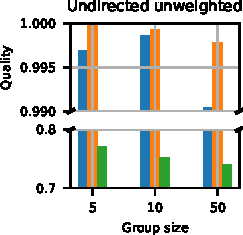
\includegraphics[width=.49\textwidth]{./sources/plots/gh-gc-apx/quality-ilp-harmonic-high-diameter-undirected-unweighted.pdf}
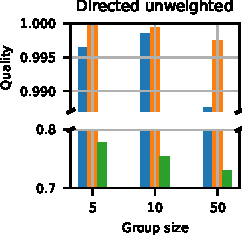
\includegraphics[width=.49\textwidth]{./sources/plots/gh-gc-apx/quality-ilp-harmonic-high-diameter-directed-unweighted.pdf}
\caption{High-diameter networks}
\label{fig:gh-gc-apx:qual-vs-opt-gh-high-diam}
\end{subfigure}

\caption{Quality relative to the optimum for group-harmonic maximization over the networks of
\Cref{tab:gh-gc-apx:small-inst-gh}, \Cref{sec:gh-gc:inst-stats}.}
\label{fig:gh-gc-apx:qual-vs-opt-gh}
\end{figure}

\Cref{fig:gh-gc-apx:qual-vs-opt-gh-cplx} shows a comparison of the solution
quality of our algorithms for group-harmonic maximization against to exact
solutions on complex networks. We observe that random groups cover unweighted
graphs reasonably well; hence, \bestrandomh already yields solutions of $>70\%$
of the optimum. This peculiarity is amplified by the fact that the networks are
rather small compared to $k$ -- they have at most \numprint{1000} vertices.
Indeed, the quality of \bestrandomh \emph{increases} with $k$ on complex
networks, a behavior that no other algorithm shows. Still, \greedyh yields
substantially better solutions in all cases: its solutions are
$>\numprint{99.5}\%$ of the optimum for all group sizes. These solutions are
further improved by \greedylsh, which yields groups with at least
$\minQualLSGRHCplxUnw$ of the optimal quality.

In high-diameter networks (\Cref{fig:gh-gc-apx:qual-vs-opt-gh-high-diam}),
\bestrandomh is not a serious competitor. Its solutions are less than $80\%$
the optimal quality. Indeed, due to the higher diameter, it is expected
that a random group of vertices is less likely to be central.
On the other hand, \greedyh and \greedylsc yield solution qualities
from $\minQualGRHRoadUnw$ and $\minQualLSGRHRoadUnw$, respectively.
For $k = 5$ in particular, solutions returned by \greedylsh have
$>\numprint{99.99}\%$ the quality of the optimal solution.

Concerning weighted high-diameter networks, the ILP solver runs
out of time or memory on nearly all instances. Tentative results
on the two remaining instances suggest that \greedyh yields solutions
that are almost optimal but, due to the small size of the dataset,
we cannot conclude definitive results.

\paragraph{Quality and Running Time on Larger Instances}
%
\begin{figure}[tb]
\begin{subfigure}[t]{\textwidth}
\centering

\includegraphics{./sources/plots/gh-gc-apx/legend-large-harmonic.pdf}
\end{subfigure}\medskip

\begin{subfigure}[t]{\textwidth}
\centering
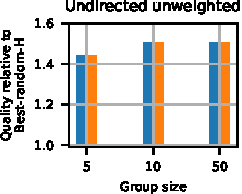
\includegraphics[width=.24\textwidth]{./sources/plots/gh-gc-apx/quality-harmonic-small-diameter-undirected-unweighted.pdf}
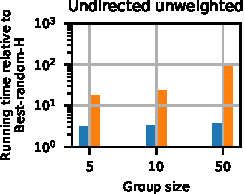
\includegraphics[width=.24\textwidth]{./sources/plots/gh-gc-apx/time-harmonic-small-diameter-undirected-unweighted.pdf}
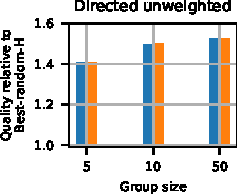
\includegraphics[width=.24\textwidth]{./sources/plots/gh-gc-apx/quality-harmonic-small-diameter-directed-unweighted.pdf}
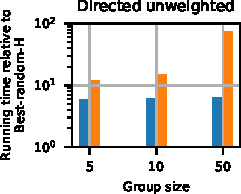
\includegraphics[width=.24\textwidth]{./sources/plots/gh-gc-apx/time-harmonic-small-diameter-directed-unweighted.pdf}
\caption{Complex networks}
\label{fig:gh-gc-apx:qual-time-gh-cplx}
\end{subfigure}\medskip

\begin{subfigure}[t]{\textwidth}
\centering
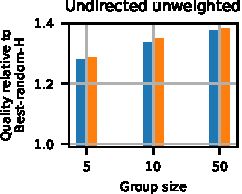
\includegraphics[width=.24\textwidth]{./sources/plots/gh-gc-apx/quality-harmonic-high-diameter-undirected-unweighted.pdf}
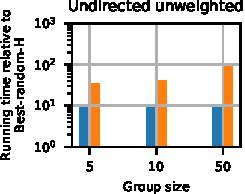
\includegraphics[width=.24\textwidth]{./sources/plots/gh-gc-apx/time-harmonic-high-diameter-undirected-unweighted.pdf}
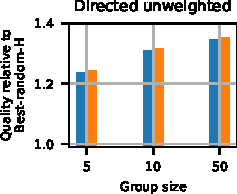
\includegraphics[width=.24\textwidth]{./sources/plots/gh-gc-apx/quality-harmonic-high-diameter-directed-unweighted.pdf}
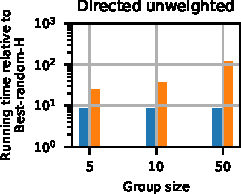
\includegraphics[width=.24\textwidth]{./sources/plots/gh-gc-apx/time-harmonic-high-diameter-directed-unweighted.pdf}
\medskip

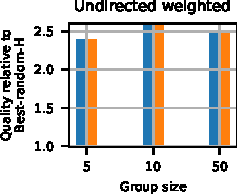
\includegraphics[width=.24\textwidth]{./sources/plots/gh-gc-apx/quality-harmonic-high-diameter-undirected-weighted.pdf}
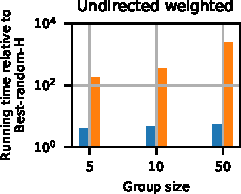
\includegraphics[width=.24\textwidth]{./sources/plots/gh-gc-apx/time-harmonic-high-diameter-undirected-weighted.pdf}
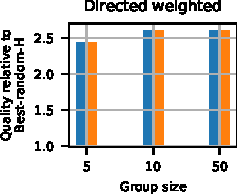
\includegraphics[width=.24\textwidth]{./sources/plots/gh-gc-apx/quality-harmonic-high-diameter-directed-weighted.pdf}
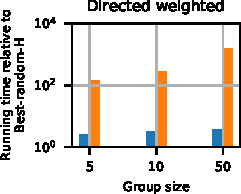
\includegraphics[width=.24\textwidth]{./sources/plots/gh-gc-apx/time-harmonic-high-diameter-directed-weighted.pdf}
\caption{High-diameter networks}
\label{fig:gh-gc-apx:qual-time-gh-high-diam}
\end{subfigure}\medskip
\caption{Quality and time \wrt \bestrandomh over the networks of \Cref{tab:gh-gc-apx:large-inst-gh}.}
\label{fig:gh-gc-apx:qual-time-gh}
\end{figure}


\Cref{fig:gh-gc-apx:qual-time-gh} summarizes quality and running time results of \greedyh and
\greedylsh (absolute running time are reported in
\Cref{tab:gh-gc-apx:time-gh-cplx,tab:gh-gc-apx:time-gh-high-diam},
\Cref{sec:gh-gc:running-times-gh}).
Due to the size of these graphs, it is not feasible to compute an ILP solution.
Thus, we use \bestrandomh as baseline. In unweighted complex networks
(\Cref{fig:gh-gc-apx:qual-time-gh-cplx}), \greedyh finds solutions with quality
(compared to \bestrandomh) from \minQualGRHRndCplxDir (with $k = 5$) to
\maxQualGRHRndCplxDir (with $k = 50$) in directed networks, and from
\minQualGRHRndCplxUnd to \maxQualGRHRndCplxUnd in undirected networks.
Compared to \greedyh, and \greedylsh is not competitive: it improves the
quality by at most \maxQualImprLSGRHCplxDir while being \minSlowdLSGRHCplxDir
to \maxSlowdLSGRHCplxDir slower.

\greedyh achieves even better results in high-diameter networks: in weighted
directed high-diameter networks (\Cref{fig:gh-gc-apx:qual-time-gh-high-diam}),
\greedyh's quality is
\minQualGRHRndRoadDirWei to \maxQualGRHRndRoadDirWei
\bestrandomh's while being just \minSlowdGRHRoadDirWei to \maxSlowdGRHRoadDirWei
slower.
Concerning \greedylsh, it is even less competitive than in complex networks:
it improves \greedyh's quality by at most \maxQualImprLSGRHRoadDirWei, while being
\minSlowdLSGRHRoadDirWei to \maxSlowdLSGRHRoadDirWei slower. Results are more
promising in high-diameter unweighted networks: here \greedylsh improves
\greedyh's quality by \minQualImprLSGRHRoadUnw to \maxQualImprLSGRHRoadUnw
while being \minSlowdGRHRoadUnw to \maxSlowdGRHRoadUnw slower.


\subsection{Group-Closeness Maximization}
\label{sec:gh-gc:exp-gc-max}
\paragraph{Comparison to Exact ILP Solutions}
%
\begin{figure}[tb]
\centering
\begin{subfigure}[t]{\textwidth}
\centering

\includegraphics{./sources/plots/gh-gc-apx/legend-exact-closeness.pdf}
\end{subfigure}\smallskip

\begin{subfigure}[t]{\textwidth}
\centering
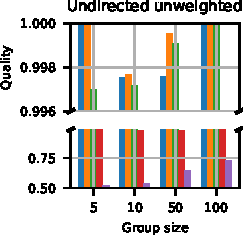
\includegraphics[width=.24\textwidth]{./sources/plots/gh-gc-apx/quality-ilp-small-diameter-undirected-unweighted.pdf}
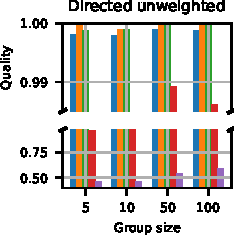
\includegraphics[width=.24\textwidth]{./sources/plots/gh-gc-apx/quality-ilp-small-diameter-directed-unweighted.pdf}
\caption{Complex networks}
\label{fig:gh-gc-apx:qual-vs-opt-gc-cplx}
\end{subfigure}\medskip

\begin{subfigure}[t]{\textwidth}
\centering
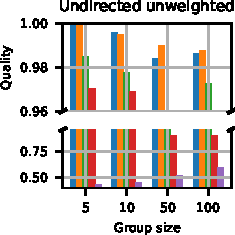
\includegraphics[width=.24\textwidth]{./sources/plots/gh-gc-apx/quality-ilp-high-diameter-undirected-unweighted.pdf}
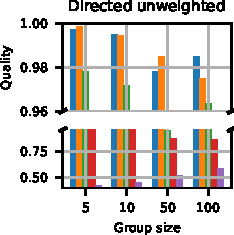
\includegraphics[width=.24\textwidth]{./sources/plots/gh-gc-apx/quality-ilp-high-diameter-directed-unweighted.pdf}
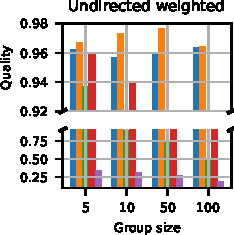
\includegraphics[width=.24\textwidth]{./sources/plots/gh-gc-apx/quality-ilp-high-diameter-undirected-weighted.pdf}
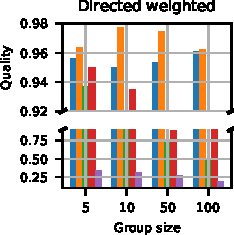
\includegraphics[width=.24\textwidth]{./sources/plots/gh-gc-apx/quality-ilp-high-diameter-directed-weighted.pdf}
\caption{High-diameter networks}
\label{fig:gh-gc-apx:qual-vs-opt-gc-high-diam}
\end{subfigure}

\caption{Quality relative to the optimum over the networks of
\Cref{tab:gh-gc-apx:small-inst-gc}.}
\label{fig:gh-gc-apx:qual-vs-opt-gc}
\end{figure}


\Cref{fig:gh-gc-apx:qual-vs-opt-gc} summarizes the quality of our local search algorithms
form group-closeness maximization and the competitors relative to the optimum.

Concerning unweighted complex networks (\Cref{fig:gh-gc-apx:qual-vs-opt-gc-cplx}),
in the directed case, for groups of size 5 \greedylsc is the only algorithm achieving
optimal solutions, while for the remaining group sizes it yields solutions with nearly
the same quality as \greedyc. In the undirected case, \greedylsc and \gslsc achieve
solutions with at least \minQualLSGRCplxUnw
and \minQualLSGSCplxUnw the optimal quality, respectively. For $k = 5$ and $k =
100$ in particular, they achieve optimal solutions.

In high-diameter networks (\Cref{fig:gh-gc-apx:qual-vs-opt-gc-high-diam}), our
local search algorithms always achieve better results than \greedyc and \gs. The
best results are on unweighted graphs: here \greedylsc and \gslsc yield
solutions at least \minQualLSGRRoadUnw and \minQualLSGSRoadUnw away from
optimality, respectively.

Interestingly, the quality of \greedylsc is often higher that \gslsc,
especially in complex networks and high-diameter weighted networks.
We conjecture that local search has a narrower improvement margin on
\gs solutions compared to \greedyc solutions since \gs is based
on local search as well.

\paragraph{Quality and Running Time on Larger Instances}
%
\begin{figure}[tb]
\begin{subfigure}[t]{\textwidth}
\centering

\includegraphics{./sources/plots/gh-gc-apx/legend-quality-closeness.pdf}
\end{subfigure}\medskip

\begin{subfigure}[t]{\textwidth}
\centering
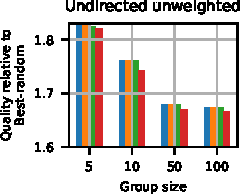
\includegraphics[width=.24\textwidth]{./sources/plots/gh-gc-apx/quality-small-diameter-undirected-unweighted.pdf}
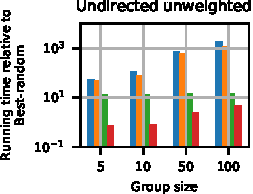
\includegraphics[width=.24\textwidth]{./sources/plots/gh-gc-apx/time-small-diameter-undirected-unweighted.pdf}
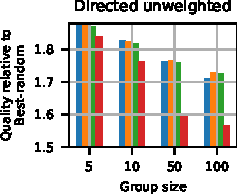
\includegraphics[width=.24\textwidth]{./sources/plots/gh-gc-apx/quality-small-diameter-directed-unweighted.pdf}
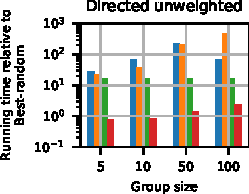
\includegraphics[width=.24\textwidth]{./sources/plots/gh-gc-apx/time-small-diameter-directed-unweighted.pdf}
\caption{Complex networks}
\label{fig:gh-gc-apx:qual-time-gc-cplx}
\end{subfigure}\medskip

\begin{subfigure}[t]{\textwidth}
\centering
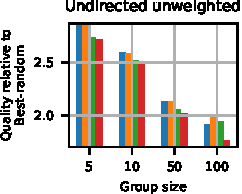
\includegraphics[width=.24\textwidth]{./sources/plots/gh-gc-apx/quality-high-diameter-undirected-unweighted.pdf}
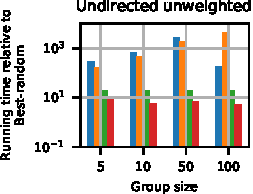
\includegraphics[width=.24\textwidth]{./sources/plots/gh-gc-apx/time-high-diameter-undirected-unweighted.pdf}
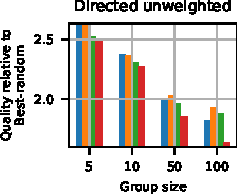
\includegraphics[width=.24\textwidth]{./sources/plots/gh-gc-apx/quality-high-diameter-directed-unweighted.pdf}
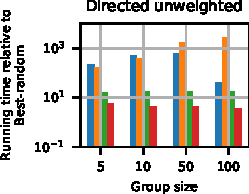
\includegraphics[width=.24\textwidth]{./sources/plots/gh-gc-apx/time-high-diameter-directed-unweighted.pdf}
\medskip

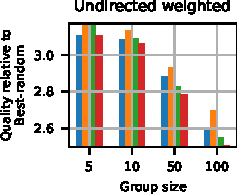
\includegraphics[width=.24\textwidth]{./sources/plots/gh-gc-apx/quality-high-diameter-undirected-weighted.pdf}
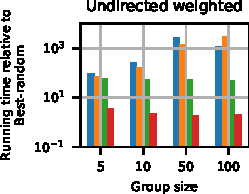
\includegraphics[width=.24\textwidth]{./sources/plots/gh-gc-apx/time-high-diameter-undirected-weighted.pdf}
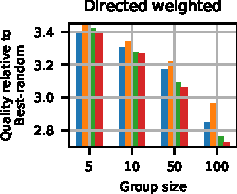
\includegraphics[width=.24\textwidth]{./sources/plots/gh-gc-apx/quality-high-diameter-directed-weighted.pdf}
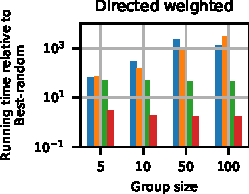
\includegraphics[width=.24\textwidth]{./sources/plots/gh-gc-apx/time-high-diameter-directed-weighted.pdf}
\caption{High-diameter networks}
\label{fig:gh-gc-apx:qual-time-gc-high-diam}
\end{subfigure}\medskip
\caption{Quality and time \wrt \bestrandomc over the networks of \Cref{tab:gh-gc-apx:large-inst-gc}.}
\label{fig:gh-gc-apx:qual-time-gc}
\end{figure}

In \Cref{fig:gh-gc-apx:qual-time-gc} we report the quality and running time of \gslsc,
\greedylsc, \greedyc, and \gs compared to \bestrandomc (absolute running times are
reported in \Cref{tab:gh-gc-apx:time-gc-cplx,tab:gh-gc-apx:time-gc-high-diam},
\Cref{sec:gh-gc:running-times-gc}).
%
In terms of quality, our local search algorithms always reach the best results
in all our experiments: in directed complex networks
(right of \Cref{fig:gh-gc-apx:qual-time-gc-cplx}), \gslsc, \greedylsc, and \greedyc
yield similar quality, while \gs has consistently the lowest quality.
%
On the other hand, quality can be traded for running time: \gs is the fastest
algorithm -- even faster than \bestrandomc for small group sizes -- \greedyc
is no average \avgSpeedGreedyCplxUnw
slower than \bestrandomc (average among all $k$), whereas \gslsc and
\greedylsc are respectively \minSpeedGSLSCplxUnw to \maxSpeedGSLSCplxUnw, and
\minSpeedGRLSCplxUnw to \maxSpeedGRLSCplxUnw slower than \bestrandomc.
%
Interestingly, for small group sizes \greedylsc is often faster than \gslsc,
and vice versa for larger groups. This is likely due to the difference
between \gs and \greedyc solutions: \greedyc aims to maximize the objective
function regardless of the group size, while for \gs the group size determines
how many vertices are consecutively added and removed in a single iteration.
Therefore, for larger groups, \gs solutions need less swaps to reach a global
optimum than \greedyc solutions.

In high-diameter networks (\Cref{fig:gh-gc-apx:qual-time-gc-high-diam}),
\greedylsc often achieves the
highest quality faster than \gslsc for all group sizes but 100.

\subsection{Parallel Scalability}
%
\begin{figure}[tb]
\centering
\begin{subfigure}[t]{\textwidth}
\centering

\includegraphics{./sources/plots/gh-gc-apx/legend-par-speedup.pdf}
\end{subfigure}\smallskip

\begin{subfigure}[t]{\textwidth}
\centering
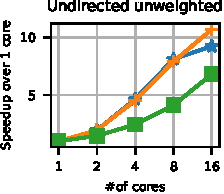
\includegraphics[width=.24\textwidth]{./sources/plots/gh-gc-apx/par-speedup-small-diameter-undirected-unweighted.pdf}
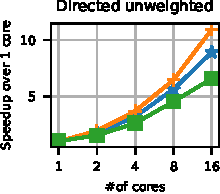
\includegraphics[width=.24\textwidth]{./sources/plots/gh-gc-apx/par-speedup-small-diameter-directed-unweighted.pdf}
\caption{Complex networks}
\end{subfigure}\medskip

\begin{subfigure}[t]{\textwidth}
\centering
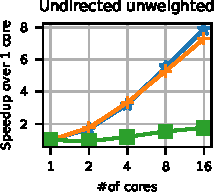
\includegraphics[width=.24\textwidth]{./sources/plots/gh-gc-apx/par-speedup-high-diameter-undirected-unweighted.pdf}
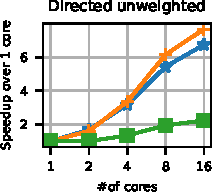
\includegraphics[width=.24\textwidth]{./sources/plots/gh-gc-apx/par-speedup-high-diameter-directed-unweighted.pdf}
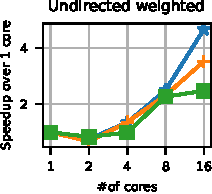
\includegraphics[width=.24\textwidth]{./sources/plots/gh-gc-apx/par-speedup-high-diameter-undirected-weighted.pdf}
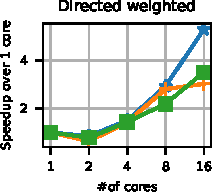
\includegraphics[width=.24\textwidth]{./sources/plots/gh-gc-apx/par-speedup-high-diameter-directed-weighted.pdf}
\caption{High-diameter networks}
\label{fig:gh-gc-apx:par-speed-high-diam}
\end{subfigure}

\caption{Parallel scalability of our algorithms for group-closeness maximization
over the networks of \Cref{tab:gh-gc-apx:large-inst-gc}, \Cref{sec:gh-gc:inst-stats}.}
\label{fig:gh-gc-apx:par-speed}
\end{figure}

Strong scaling plots for \gslsc, \greedylsc, and \greedyc are reported in
\Cref{fig:gh-gc-apx:par-speed}. On average, our local search algorithms scale
better than \greedyc on both complex and high-diameter networks. This is not
surprising: local search needs to evaluate at least $k(n - k)$ swaps,
which is a highly parallel operation, and often much more expensive than
running \greedyc.

On high-diameter networks in particular (\Cref{fig:gh-gc-apx:par-speed-high-diam}),
\greedyc has a poor parallel scalability; we conjecture that, since closeness
centrality distinguishes vertices in high-diameter networks better than in
complex networks~\cite[Ch. 7]{newman2018networks}, \greedyc needs to evaluate
only few vertices per iteration before finding the vertex with highest marginal
gain. In that case, multiple cores do not speed this process up significantly.


\section{Conclusions}
%
This chapter investigated engineering aspects of
approximating  two group centrality maximization problems, namely,
group-harmonic maximization and group-closeness maximization. We illustrated
how to efficiently implement greedy and local search approximation algorithms
and presented the results of a detailed experimental study. Our experiments
suggest that the quality of both the greedy and the local search algorithms
come very close to the optimum. This finding is consistent with the theoretical
results illustrated in Ref.~\cite{DBLP:conf/alenex/AngrimanBDGGM21}, which
assess that, in most cases, these algorithms have good approximation
guarantees. Interestingly, the two methods also perform well on directed
instances for group-closeness maximization despite the hardness of
approximation results which holds for this class of instances.

On the other hand, the quality guarantees come with a cost in running time.
Concerning group-harmonic maximization, the results presented
in~\Cref{sec:gh-gc:exp-gh-max} suggest that, despite the better approximation
guarantees, our local search algorithm is not competitive compared to
our greedy algorithm. In comparison to \greedyh, \greedylsh is \minSlowdLSGRHCplxDir
to \maxSlowdLSGRHRoadDirWei slower and yields solutions that improve
\greedyh solutions only by a thin margin. Hence, in a practical scenario,
we recommend using the greedy algorithm.

For group-closeness maximization, we conclude that, unlike the group-harmonic
case, our local search approximation algorithms are not dominated by
existing greedy~\cite{DBLP:conf/alenex/BergaminiGM18} and local search
(see \Cref{ch:group-closeness-local-search}) heuristics.
Despite being one to two orders of magnitude slower, results in
\Cref{fig:gh-gc-apx:qual-time-gc} convey that our \gslsc and \greedylsc
algorithms (especially the latter) improve \greedyc and \gs solutions
by a solid margin. Therefore, among the available algorithms, \greedylsc is the
most amenable choice for applications dealing with networks of moderate size
and where solution quality is of highest concern.
